\documentclass[11pt]{article}

%%%%%%%%%%%%%%%%
% Packages
%%%%%%%%%%%%%%%%

\usepackage[top=1cm,bottom=1.1cm,left=1.25cm,right= 1.25cm]{geometry}
\usepackage[parfill]{parskip}
\usepackage{graphicx, fontspec, xcolor,multicol, enumitem, setspace, amsmath, changepage}
\DeclareGraphicsRule{.tif}{png}{.png}{`convert #1 `dirname #1`/`basename #1 .tif`.png}

%%%%%%%%%%%%%%%%
% User defined colors
%%%%%%%%%%%%%%%%

% Pantone 2015 Fall colors
% http://iwork3.us/2015/02/18/pantone-2015-fall-fashion-report/
% update each semester or year

\xdefinecolor{custom_blue}{rgb}{0, 0.32, 0.48} % FROM SPRING 2016 COLOR PREVIEW
\xdefinecolor{custom_darkBlue}{rgb}{0.20, 0.20, 0.39} % Reflecting Pond  
\xdefinecolor{custom_orange}{rgb}{0.96, 0.57, 0.42} % Cadmium Orange
\xdefinecolor{custom_green}{rgb}{0, 0.47, 0.52} % Biscay Bay
\xdefinecolor{custom_red}{rgb}{0.58, 0.32, 0.32} % Marsala

\xdefinecolor{custom_lightGray}{rgb}{0.78, 0.80, 0.80} % Glacier Gray
\xdefinecolor{custom_darkGray}{rgb}{0.35, 0.39, 0.43} % Stormy Weather

%%%%%%%%%%%%%%%%
% Color text commands
%%%%%%%%%%%%%%%%

%orange
\newcommand{\orange}[1]{\textit{\textcolor{custom_orange}{#1}}}

% yellow
\newcommand{\yellow}[1]{\textit{\textcolor{yellow}{#1}}}

% blue
\newcommand{\blue}[1]{\textit{\textcolor{blue}{#1}}}

% green
\newcommand{\green}[1]{\textit{\textcolor{custom_green}{#1}}}

% red
\newcommand{\red}[1]{\textit{\textcolor{custom_red}{#1}}}

%%%%%%%%%%%%%%%%
% Coloring titles, links, etc.
%%%%%%%%%%%%%%%%

\usepackage{titlesec}
\titleformat{\section}
{\color{custom_blue}\normalfont\Large\bfseries}
{\color{custom_blue}\thesection}{1em}{}
\titleformat{\subsection}
{\color{custom_blue}\normalfont}
{\color{custom_blue}\thesubsection}{1em}{}

\newcommand{\ttl}[1]{ \textsc{{\LARGE \textbf{{\color{custom_blue} #1} } }}}

\newcommand{\tl}[1]{ \textsc{{\large \textbf{{\color{custom_blue} #1} } }}}

\usepackage[colorlinks=false,pdfborder={0 0 0},urlcolor= custom_orange,colorlinks=true,linkcolor= custom_orange, citecolor= custom_orange,backref=true]{hyperref}

%%%%%%%%%%%%%%%%
% Instructions box
%%%%%%%%%%%%%%%%

\newcommand{\inst}[1]{
\colorbox{custom_blue!20!white!50}{\parbox{\textwidth}{
	\vskip10pt
	\leftskip10pt \rightskip10pt
	#1
	\vskip10pt
}}
\vskip10pt
}

%%%%%%%%%%%
% App Ex number    %
%%%%%%%%%%%

% DON'T FORGET TO UPDATE

\newcommand{\appno}[1]
{5.3}

%%%%%%%%%%%%%%
% Turn on/off solutions       %
%%%%%%%%%%%%%%

% Off
\newcommand{\soln}[2]{$\:$\\ \vspace{#1}}{}

%%% On
%\newcommand{\soln}[2]{\textit{\textcolor{custom_red}{#2}}}{}

%%%%%%%%%%%%%%%%
% Document
%%%%%%%%%%%%%%%%

\begin{document}
\fontspec[Ligatures=TeX]{Helvetica Neue Light}

Dr. \c{C}etinkaya-Rundel \hfill Sta 101: Data Analysis and Statistical Inference \\
Duke University - Department of Statistical Science \hfill \\

\ttl{Application exercise \appno{}: \\
Chi-square testing}

\inst{$\:$ \\
Team name: \rule{10cm}{0.5pt} \\
$\:$ \\
Lab section: $\qquad$ 8:30 $\qquad$ 10:05 $\qquad$ 11:45 $\qquad$ 1:25 $\qquad$ 3:05 \\
$\:$ \\
Write your responses in the spaces provided below. WRITE LEGIBLY and SHOW ALL WORK! 
Only one submission per team is required. One team will be randomly selected and their 
responses will be discussed and graded. Concise and coherent are best!}

%%%%%%%%%%%%%%%%%%%%%%%%%%%%%%%%%%%%

\section*{Country on track?}

The American National Election Studies (ANES) aims to inform explanations of election outcomes 
by providing data that support rich hypothesis testing, maximize methodological excellence, measure 
many variables, and promote comparisons across people, contexts, and time. In this question we will 
focus on two variables from the 2012 ANES dataset: 
\begin{itemize}
\item region (levels: Northeast, North Central, South, and West), and
\item whether the respondent feels things in this country are generally going in the right direction 
or things have pretty seriously gotten off on the wrong track.
\end{itemize}
To keep calculations simple we will work with a random sample of 500 respondents from the ANES 
dataset. The distribution of responses are as follows:

\begin{minipage}[c]{0.4\textwidth}
\begin{center}
\begin{tabular}{rrr|r}
  \hline
 & Right  & Wrong  &  \\ 
 &  Direction &  Track & Total \\ 
  \hline
Northeast & 29 & 54 & 83 \\ 
  North Central & 44 & 77 & 121 \\ 
  South & \textit{\textbf{62}} & 131 & 193 \\ 
  West & 36 & 67 & 103 \\ 
\hline
  Total & 171 & 329 & 500 \\ 
   \hline
\end{tabular}
\end{center}
\end{minipage}
\begin{minipage}[c]{0.6\textwidth}
\begin{center}
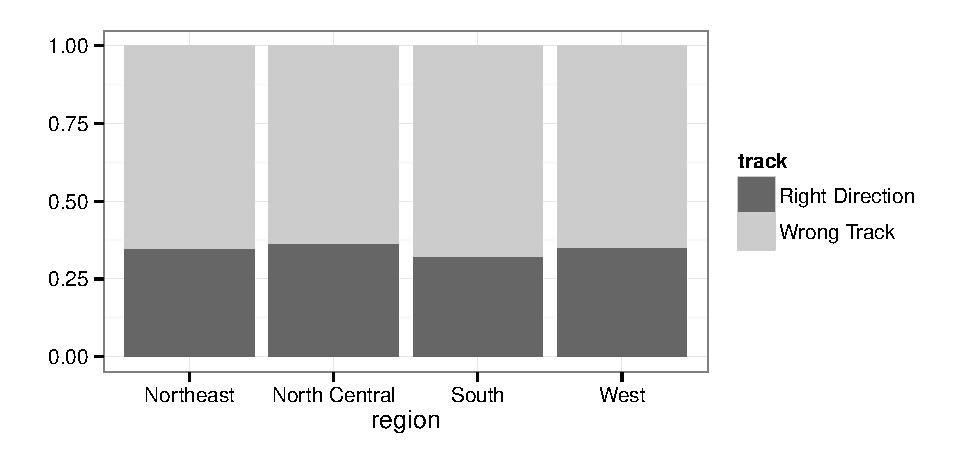
\includegraphics[width=\textwidth]{figures/anes_mosaic.pdf}
\end{center}
\end{minipage}

\pagebreak

\textbf{Part 1: Region:} 

According to the 2010 Census, 18\% of US residents live in the Northeast, 22\% live in the North 
Central region, 37\% live in the South, and 23\% live in the West. Evaluate whether the ANES sample 
is representative of the population distribution of US residents. Make sure to clearly state the hypotheses, 
check conditions, calculate the appropriate test statistic and the p-value, and make your conclusion in context 
of the data. \textbf{Also} comment on what your conclusion says about whether or not this sample can be 
considered to be representative of the US population with respect to regional population distribution. \\

Hypotheses:
\soln{1.5cm}{$H_0$: The sample distribution of regions follows the census distribution. \\
$H_A$: The sample distribution of regions does not follow the census distribution.}

Conditions:
\soln{4cm}{}

Test statistic:
\soln{3cm}{
$\chi^2 = \frac{(83 - 90)^2}{90} + \frac{(121 - 110)^2}{110} + \frac{(193 - 185)^2}{185} + \frac{(103 - 115)^2}{115} \approx 3.24$ \\
$df = 4 - 1 = 3$}

p-value:
\soln{1cm}{$p-value > 0.3$}

Decision (circle one):  $\qquad$ Reject $H_0$ $\qquad \qquad \qquad$ Fail to reject $H_0$ \\
$\:$ \\

Conclusion in context of the data:
\soln{2cm}{The data do not provide convincing evidence that the sample distribution of regions does not follow the 
census distribution.}

Comment on representative sample:
\soln{2cm}{The sample is likely representative since the distribution of sampled individual matches the distribution 
regional population distribution.}

%
\pagebreak

\textbf{Region and direction:} 

\begin{enumerate}

\item In evaluating the relationship between region and feeling about the direction things 
are going in the country, what is the response variable and what is the explanatory variable?
\begin{itemize}
\item[-] response: \soln{0.2cm}{direction} \\
\item[-] explanatory: \soln{0.2cm}{region} \\
\end{itemize}

\item What are the hypotheses for evaluating this relationship?

\soln{3cm}{$H_0:$ Region and opinion on direction are independent. \\
$H_A:$ Region and opinion on direction are dependent. \\
}

\item Speculate on whether you would expect to reject or not reject the null hypothesis based on the 
segmented bar chart shown above. Explain your reasoning in at most two sentences. Note that in
this question you are not being asked to actually carry out the hypothesis test.

\soln{3cm}{No, \\
P(right direction $|$ each level of the region variable) is roughly equal, chances are we won't reject $H_0$.}

\item If in fact the null hypothesis is true, how many Southerners would we expect to respond that 
they feel things in this country are generally going in the right direction?

\soln{3cm}{$E = \frac{193 \times 171}{500} = 66.006$}

\item What is the contribution of this cell (South \& Right direction) to the test statistic?

\soln{3cm}{$\frac{(62 - 66.006)^2}{66.006} = 0.24313$}

\item The $\chi^2$ statistic for this test is 0.667. Determine is the degrees of freedom associated with this
test statistic and the p-value for this test.

\soln{3cm}{$df = (R - 1) \times (C - 1) = 3 \times 1 = 3$ \\
$p-value = 0.8809$ (or something around this if using the table)
}

\item What is the conclusion of the hypothesis test?

\soln{1cm}{Fail to reject $H_0$. The data do not provide convincing evidence for a relationship
between region and feeling about the direction things are going in the country.
}

\end{enumerate}

\end{document}